% =====================================================================
% Appendix C (app:scorer): scorer specification and metric validation
% (one-column appendix).
% Floats: Table A3 (tables/tab_sanity.tex), Table A7 (tables/tab_validity.tex),
% Fig. A4 (fig:sim2real, defined below).
% Implemented in the released scorer: submission format, normalisation,
% resegmentation, oracle turn-ID mode, BLEU, chrF, StreamLAAL, EndOffset,
% empty turns, wrong-language words given turn IDs. Everything else is
% planned and carries a \draftnote. Sanity-run numbers are preliminary (\prelim).
% Notation as in Secs. 3-4: b_n, e_n, L_n, r_n, h_n, tau_{n,j}, d_{n,j}, rho_n, J_n.
% Holds what Sec. 4 leaves out: normalisation, resegmentation algorithm,
% oracle mode (final results strip turn IDs), aggregation, penalised and
% matched-word variants, metric credits (SimulEval EndOffset/StartOffset,
% Seamless), the 540-of-554 switch caveat, the detector, transcript metrics,
% meta-evaluation and rank agreement (tau_b within direction x wrapper
% strata, averaged; n reported; threshold fixed before the test runs).
% Open user decisions, not applied: a time constraint on resegmentation,
% a "switch cost" metric, an "overrun rate" metric, COMET on raw Syn text,
% a minimum piece length for the language-ID rule, a TAXI-TTS control.
% =====================================================================
\section{Scorer Specification and Metric Validation}\label{app:scorer}

This appendix specifies \scorer precisely enough to reimplement it and describes how we test that its metrics measure what they are meant to measure. As in \cref{sec:task,sec:bench}, turn $n$ of a session of duration $T$ has speaker $s_n$, interval $[b_n,e_n]$, duration $L_n=e_n-b_n$ and a reference translation $r_n$ of $|r_n|$ words.
\draftnote{the released scorer implements the submission format, normalisation, resegmentation, oracle mode, BLEU, chrF, \laal, \eo, empty turns and wrong-language words given gold turn IDs; a pinned num2words, COMET, switch latency, the length ratio, the wrong-direction detector, the latency variants, the bootstrap and all transcript and speaker metrics are planned}

\subsection{Submission, clocks and normalisation}

\paragraph{Submission.}
A system submits one JSON line per committed piece with four fields: session ID, output language, emission time $t$ in seconds from the start of \texttt{mix.wav}, and text. The output language selects the direction (English output translates German speech), so no speaker or direction label is needed. Pieces are never retracted, and every line counts as committed. The scorer sorts the pieces of each session by emission time, keeping file order for ties, splits each normalised piece into words and gives every word the time of its piece. An optional gold turn ID per piece selects the oracle mode described below. Further fields are kept, and any of them can serve as the clock; pieces of unknown sessions are reported and ignored.

\paragraph{Clocks.}
On the ideal clock, $t$ is the audio consumed when the piece is committed; the computation-aware clock \citep{ma2020simulmt} adds processing time measured on fixed hardware (\cref{tab:ca-latency}). Unlike SimulEval \citep{ma2020simuleval}, which runs a policy on each source segment, \scorer sees only committed pieces and their times, so they can come from any streaming harness, such as simulstream \citep{gaido2025simulstream}, or from a unified model. On \taxi, turn intervals include the 0.1\,s margins of energy trimming (\cref{app:taxi}), which can move the reference points of every latency metric by up to about 0.1\,s.

\paragraph{Normalisation.}
Hypotheses and references are normalised alike, to the style of the TAXI references (lowercase, unpunctuated, numbers in words): (i)~Unicode NFC; (ii)~each number, i.e., a digit string with an optional decimal part, is spelled out with num2words in the output language, reading a decimal comma as a decimal point in German and dropping commas as thousands separators in the other languages; (iii)~lowercasing; (iv)~every character other than a letter, a digit, whitespace or a word-internal apostrophe becomes a space; (v)~splitting at whitespace. The scorer depends on a pinned num2words version, because without the package step~(ii) would be skipped silently.
\draftnote{planned: pinning num2words; the released scorer lists it only as an optional dependency (version 0.5 or later) and skips step (ii) silently if it is missing}

\paragraph{Quality.}
Per direction, BLEU \citep{papineni2002bleu} and chrF \citep{popovic2015chrf} are sacreBLEU corpus scores \citep{post2018call} over the turns of that direction, with default settings except for sacreBLEU's Korean tokenizer for BLEU into Korean; we report the signatures and two decimals. An empty turn enters as an empty hypothesis and lowers both scores. COMET with the wmt22-comet-da model \citep{rei2020comet,rei2022comet} scores the same resegmented turns, with the gold transcript as the source. A per-turn file holds each turn's source, hypothesis, reference and latencies; for \taxi, only per-turn scores keyed by turn ID are released (\cref{app:repro}).
\draftnote{planned: COMET inside the scorer and the Korean tokenizer; the released scorer leaves COMET to external tools reading the per-turn file}

\subsection{Resegmentation and oracle mode}

For each session and output language $\lambda$, \scorer assigns the hypothesis words to the turns $\mathcal{N}_\lambda$ that are translated into $\lambda$, with the minimum-edit-distance criterion of mwerSegmenter \citep{matusov2005evaluating} as used in stream-level evaluation \citep{iranzosanchez2021stream,papi2024streamatt}:
\begin{enumerate}
  \item order the hypothesis words $w_1,\dots,w_M$ by emission time;
  \item concatenate the normalised references $r_n$, $n\in\mathcal{N}_\lambda$, in dialogue order into $u_1,\dots,u_K$, and record the turn $o(k)$ of each reference word $u_k$;
  \item align $w_{1:M}$ to $u_{1:K}$ by word-level Levenshtein alignment with unit costs; on ties, the backtrace prefers a match or substitution to an insertion, and an insertion to a deletion;
  \item assign each $w_i$ aligned to some $u_k$, as a match or a substitution, to turn $o(k)$; assign each inserted word to the turn of the preceding aligned word or, if it precedes all aligned words, to the turn of the first aligned word.
\end{enumerate}
Turn $n$ thus receives the words $h_n$, with emission times $\tau_{n,1}\le\dots\le\tau_{n,|h_n|}$, and is empty if $h_n$ is empty. Resegmentation looks only at text, so a word can land in a turn that begins after the word was emitted, and latency on resegmented output inherits a segmentation-related bias \citep{polak2025better}.

\paragraph{Oracle mode.}
If every piece of a session and direction carries a gold turn ID, the scorer skips resegmentation and assigns words to their turns directly; words whose ID is not a turn of direction $\lambda$ count as wrong-language words and are not scored. This mode is only a diagnostic (\cref{sec:task}): scoring the same output both ways measures how much resegmentation alone moves the scores. Final results are resegmented, with any turn IDs removed from the hypotheses first; the preliminary rows of \cref{tab:main} were scored in oracle mode and will be re-scored.

\subsection{Latency}

For a non-empty turn $n$, let $d_{n,j}=\max(0,\tau_{n,j}-b_n)$ be the delay of its $j$-th word from the turn start, $\rho_n=L_n/\max(|h_n|,|r_n|)$ the rate, and $J_n$ the first $j$ with $d_{n,j}\ge L_n$, or $|h_n|$ if there is none. Then
\begin{align}
  \mathrm{StreamLAAL}_n &= \frac{1}{J_n}\sum_{j=1}^{J_n}\bigl(d_{n,j}-(j-1)\,\rho_n\bigr), \label{eq:app-laal}\\
  \mathrm{EndOffset}_n &= \tau_{n,|h_n|}-e_n, \label{eq:app-eo}\\
  \mathrm{SwitchLatency}_n &= d_{n,1}\qquad\text{for } n>1 \text{ with } s_n\neq s_{n-1}. \label{eq:app-switch}
\end{align}
\Cref{eq:app-laal} is LAAL \citep{papi2022overgeneration}, the length-adaptive form of Average Lagging \citep{ma2019stacl}, applied to resegmented turns, i.e., \laal \citep{papi2024streamatt}. Two cases show what the metrics separate. If a turn's translation is committed at $e_n$, every delay equals $L_n$, so $J_n=1$, $\mathrm{StreamLAAL}_n=L_n$ and $\mathrm{EndOffset}_n=0$: offline systems on oracle turns score the mean turn duration, 4.624\,s for \ende and 3.086\,s for \deen on \taxi. If instead the $j$-th of the $|r_n|$ reference words is committed at $b_n+jL_n/|r_n|$, then $\mathrm{StreamLAAL}_n=L_n/|r_n|$, the duration of one word, while $\mathrm{EndOffset}_n$ is still 0. \laal thus measures the lag within a turn and \eo the wait after it. \eo is negative if a turn's output ends before the speaker does, through anticipation or truncation, so we always report it with quality and length ratio. Neither waiting metric is new: \eo is SimulEval's EndOffset, the delay of the last output after the end of the source \citep{ma2020simuleval}, which SeamlessStreaming also reports as its ending offset \citep{seamless2023seamless}, computed here per turn; switch latency (\cref{eq:app-switch}) is SimulEval's StartOffset, the delay of the first output, taken only at turns that change direction. It is undefined for the first turn of a session, so the two single-turn \taxi sessions contribute none; and as 540 of the 554 later \taxi turns follow a speaker change, switch latency on \taxi is close to the first-word delay of all later turns.

\paragraph{Aggregation.}
Per direction, we report the mean, median and 90th percentile over non-empty turns, to three decimals. The median averages the two middle values of an even count, and the 90th percentile of $m$ values is the sorted value at the 0-based index $\min(m-1,\lfloor 0.9m\rfloor)$. The empty-turn rate is reported next to every latency.

\paragraph{Penalised variant.}
Averaging over non-empty turns lets a system improve its latency by dropping hard turns. The penalised variant therefore scores an empty turn as if its whole reference were committed at the session end: $\mathrm{EndOffset}_n=T-e_n$ and $\mathrm{StreamLAAL}_n=\mathrm{SwitchLatency}_n=T-b_n$. On the ideal clock no piece comes later than $T$, so these are the worst values any output can obtain, and dropping a turn never lowers its latency.

\paragraph{Exactly matched words.}
Unrelated output can lower \laal (row~2 of \cref{tab:sanity}); one mechanism is that a word assigned to a turn that begins after the word was emitted gets delay 0. We therefore also report \cref{eq:app-laal,eq:app-eo} with $h_n$ restricted to the words that exactly match their aligned reference word, so that unrelated words cannot contribute.
\draftnote{planned: switch latency, the penalised variant and the matched-word variant}

\subsection{Errors and auxiliary outputs}

\paragraph{Empty turns and length ratio.}
A turn is empty if no word is assigned to it. Per direction, we report the share of empty turns and the ratio of hypothesis to reference words.
\draftnote{planned: the length ratio; the released scorer reports only the numbers of turns and of empty turns}

\paragraph{Wrong-direction words.}
In oracle mode, wrong-direction words are the wrong-language words defined above. Without turn IDs, a piece $(t_i,\lambda_i,y_i)$ is checked against the turns open at its emission time, $\mathcal{A}(t_i)=\{n: b_n\le t_i\le e_n+W\}$, with a window $W$ fixed before any system is scored. All words of the piece are wrong-direction words if
(a)~\emph{wrong channel}: $\mathcal{A}(t_i)$ is non-empty and all its turns are spoken in $\lambda_i$, so no open turn needs a translation into $\lambda_i$;
(b)~\emph{wrong language}: a text language identifier restricted to the session's two languages assigns $y_i$ to the language other than $\lambda_i$; or
(c)~\emph{copy-through}: $y_i$ is closer to the transcript of an open turn spoken in $\lambda_i$ than to the reference of every open turn translated into $\lambda_i$, where the distance from $y_i$ to a text is the smallest word edit distance between $y_i$ and a span of that text, divided by the length of $y_i$.
Under turn-end overlap, turns in both languages are open at once, so (a) cannot fire and (b) and (c) decide. Rows~2 and~8 of \cref{tab:sanity} test (b) and (c), and the delayed rows check that late but correct output is not flagged. We report wrong-direction words as a percentage of all committed words and compare the detector with the oracle-mode count wherever turn IDs exist.
\draftnote{planned: the detector, its window $W$ and the text language identifier; the released scorer counts wrong-language words only given gold turn IDs}

\paragraph{Transcripts and speakers.}
For systems with a transcript channel, we report WER per language after the same normalisation; cpWER \citep{watanabe2020chime}, which compares each speaker's concatenated words under the best mapping between hypothesis and reference speakers, so that arrival-order labels need no fixed identity; and its time-constrained variant tcpWER from MeetEval \citep{vonneumann2023meeteval}. For Korean, cpCER applies cpWER to characters instead of words. DER uses collars of 0 and 0.25\,s at 80\,ms resolution. The main text reports WER, cpWER (cpCER on \syn \pair{Ko}{En}) and DER (\cref{tab:aux}); tcpWER and DER without a collar are in \cref{app:results}.
\draftnote{planned}

\paragraph{Speaker-attributed BLEU.}
DiariST scores translations per speaker after mapping hypothesis speakers to reference speakers \citep{yang2024diarist}. In \task each speaker uses one language, so the reference translations of speaker~$A$ are exactly those of direction $\ell_A\to\ell_B$. For a system that labels its translations with speakers, speaker-attributed BLEU therefore scores the same hypothesis--reference pairs as per-direction BLEU whenever every piece labelled~$A$ is in $\ell_B$ and every piece labelled~$B$ is in $\ell_A$. The two differ only on pieces whose label contradicts their language; these are attribution or direction errors, which the wrong-direction rate and cpWER already count. We therefore compute speaker-attributed BLEU only as a consistency check for systems with speaker labels.

\subsection{Metric meta-evaluation}

% =====================================================================
% Table A3 (tab:sanity): metric meta-evaluation by controlled perturbations
% of the reference output on CST-Bench-TAXI, L0 natural. Included from App. C,
% which describes how every row is constructed.
% Rows 1-2: preliminary scorer sanity runs (\prelim; to be re-run and recorded).
% All other cells are pending (\tbd). W counts words (not a percentage).
% Rows 3-5 state their delay (+0.5/+1/+2 s); the symbol Delta is avoided because
% it is the chunk length in Sec. 5 and a COMET difference in Tables 4 and 6.
% =====================================================================
\begin{table}[t]
  \caption{Metric meta-evaluation on \taxi, L0 natural: controlled perturbations of the reference translations, with the change expected for each metric fixed in advance (construction of each row in \cref{app:scorer}). Q: BLEU and chrF; L: mean \laal (s); E: mean \eo (s), both over non-empty turns; W: number of wrong-direction words; $L_n$, $|r_n|$: duration and reference length of turn $n$; $=$: unchanged; $\uparrow$\,/\,$\downarrow$: increases\,/\,decreases. $^\dagger$Preliminary; to be re-run under the final protocol. $^\ast$The current scorer counts such words only given gold turn IDs. Blank cells are pending.}
  \label{tab:sanity}
  \centering
  \footnotesize
  \setlength{\tabcolsep}{3pt}
  \begin{tabular}{@{}rllccccccc@{}}
    \toprule
    & & & \multicolumn{3}{c}{\ende} & \multicolumn{3}{c}{\deen} & \\
    \cmidrule(lr){4-6}\cmidrule(lr){7-9}
    & Perturbation & Expected change & BLEU\,/\,chrF & L & E & BLEU\,/\,chrF & L & E & W \\
    \midrule
    1  & Reference at turn end
       & \makecell[l]{Q $=100$; L $=$ mean $L_n$;\\E $=0$; W $=0$}
       & \prelim{100.0\,/\,100.0} & \prelim{4.624} & \prelim{0.0}
       & \prelim{100.0\,/\,100.0} & \prelim{3.086} & \prelim{0.0} & \prelim{0} \\
    2  & \makecell[l]{Source transcript passed\\through untranslated}
       & \makecell[l]{Q $\approx0$; L, E not below\\row 1; W $=$ all words}
       & \prelim{2.38\,/\,27.34} & \prelim{4.366} & \prelim{2.576}
       & \prelim{0.39\,/\,21.86} & \prelim{2.276} & \prelim{1.421} & \prelim{0}$^\ast$ \\
    3  & Row 1 delayed by 0.5\,s & Q $=$; L, E $+0.5$\,s; W $=0$ & \tbd & \tbd & \tbd & \tbd & \tbd & \tbd & \tbd \\
    4  & Row 1 delayed by 1\,s   & Q $=$; L, E $+1$\,s; W $=0$ & \tbd & \tbd & \tbd & \tbd & \tbd & \tbd & \tbd \\
    5  & Row 1 delayed by 2\,s   & Q $=$; L, E $+2$\,s; W $=0$ & \tbd & \tbd & \tbd & \tbd & \tbd & \tbd & \tbd \\
    6  & \makecell[l]{Reference spread evenly\\over the turn}
       & \makecell[l]{Q $=$; L $=$ mean $L_n/|r_n|$;\\E $=0$; W $=0$}
       & \tbd & \tbd & \tbd & \tbd & \tbd & \tbd & \tbd \\
    7  & \makecell[l]{Row 6 without the last\\third of each turn}
       & \makecell[l]{vs.\ row 6: Q $\downarrow$; L $=$;\\E $\downarrow$ (below 0); W $=0$}
       & \tbd & \tbd & \tbd & \tbd & \tbd & \tbd & \tbd \\
    8  & \makecell[l]{Turns merged across a\\speaker change (VAD)}
       & \makecell[l]{Q $\downarrow$; E $\uparrow$; W $\uparrow$;\\more empty turns}
       & \tbd & \tbd & \tbd & \tbd & \tbd & \tbd & \tbd \\
    9  & \makecell[l]{Output of 10\% of turns\\dropped}
       & \makecell[l]{Q $\downarrow$; L, E $\approx$ row 1;\\10\% empty turns}
       & \tbd & \tbd & \tbd & \tbd & \tbd & \tbd & \tbd \\
    10 & \makecell[l]{Rows 1, 3--7, 9 with gold\\turn IDs: largest change}
       & 0 for every metric
       & \tbd & \tbd & \tbd & \tbd & \tbd & \tbd & \tbd \\
    \bottomrule
  \end{tabular}
\end{table}


We perturb the reference output on \taxi L0 natural and check that BLEU, chrF, \laal, \eo and the wrong-direction count each move as expected while the others stay put (\cref{tab:sanity}); the expected changes are fixed in advance. COMET and switch latency are not yet in the table, as the released scorer does not compute them. Row~1 commits every reference translation at its turn end. Row~2 emits each turn's source transcript as its translation, as a system that passes speech through untranslated would. Rows~3--5 delay row~1 by 0.5, 1 and 2\,s. Row~6 commits the $j$-th reference word of turn $n$ at $b_n+jL_n/|r_n|$, and row~7 drops the last $\lfloor|r_n|/3\rfloor$ words of every turn of row~6. Row~8 simulates a VAD that merges two turns across a speaker change, at a seeded subset of speaker changes: the first turn's reference is committed at the end of the second turn, followed on the same channel by the second turn's source transcript, as if the merged segment had been routed by the first turn's language. Row~9 removes the output of a seeded 10\% of turns. Row~10 rescores rows~1, 3--7 and~9, whose words all come from the right turns, with gold turn IDs and reports the largest change. No final system result is reported until every row behaves as expected or the deviation is explained; the preliminary system results have not yet passed this check and will be re-run. We repeat the comparison of row~10 for every system run under the oracle wrapper, whose pieces carry turn IDs.

Rows~1 and~2 exist so far only as preliminary runs ($^\dagger$; to be re-run under the final protocol). Row~1 behaves as derived above: BLEU and chrF are \prelim{100.0}, \eo is \prelim{0.0}\,s, no word counts as wrong, and the mean \laal equals the mean turn duration (\prelim{4.624}\,s for \ende, \prelim{3.086}\,s for \deen). Row~2 drives BLEU down to \prelim{2.38} for \ende and \prelim{0.39} for \deen, while chrF keeps \prelim{27.34} and \prelim{21.86} from shared character n-grams. However, it \emph{lowers} the mean \laal below that of the reference (\prelim{4.366} vs.\ \prelim{4.624}\,s for \ende; \prelim{2.276} vs.\ \prelim{3.086}\,s for \deen) and raises the mean \eo to \prelim{2.576} and \prelim{1.421}\,s, presumably because resegmentation spreads the untranslated words over neighbouring turns; and without turn IDs, the current scorer counts none of these words as wrong. These two failures motivate the matched-word latency, the rule to show latency only next to quality, length ratio and empty turns, and the wrong-direction detector. In addition, five unit tests check normalisation, resegmentation, LAAL, oracle versus resegmented scoring and the command-line interface on toy sessions; for instance, an oracle hypothesis scores BLEU 100.0 with a mean \eo of 0.0\,s, and a two-word turn reaches chrF 100.0.
\draftnote{re-run rows 1--2 under the final protocol and record how the row-2 hypothesis is time-stamped}

\subsection{Rank agreement and sim-to-real validity}

% =====================================================================
% Table A7 (tab:validity): rank-agreement checks behind the validity claims
% (sim-to-real, TTS edition, silver references, render seeds, metric choice).
% Included from App. C. Nothing has been run yet: every cell is \tbd.
% tau_b is computed within direction x wrapper strata and averaged, so that
% wrapper and direction differences cannot inflate agreement (review); the
% "oracle--realistic gap" row ranks systems by their gap on each set, as the
% paper's claims rest on gaps. A TAXI-TTS control row would be a new
% experiment (user decision) and is not listed.
% =====================================================================
\begin{table}[t]
  \caption{Validity of system rankings (TAXI: \taxi; Syn: \syn; all L0 natural). Each row ranks the same systems at their main operating points in two ways; Kendall's $\tau_b$ is computed within each direction $\times$ wrapper stratum (each direction for gaps) and averaged over strata, with a 95\% CI from 2,000 session-bootstrap resamples; $n$ counts the ranked configurations. For render seeds, $\tau_b$ is the smallest pairwise value among the three renders; \cref{app:scorer} also compares their standard deviation with the CI width. Blank cells are pending.}
  \label{tab:validity}
  \centering
  \small
  \setlength{\tabcolsep}{5pt}
  \begin{tabular}{@{}llccc@{}}
    \toprule
    Comparison & Configurations compared & $n$ & Kendall's $\tau_b$ & 95\% CI \\
    \midrule
    \multicolumn{5}{@{}l}{\textit{Speech, construction and rendering (chrF rankings)}} \\
    TAXI vs.\ Syn \pair{En}{De}                 & those run on both sets  & \tbd & \tbd & \tbd \\
    \quad oracle--realistic gap                 & same, ranked by gap     & \tbd & \tbd & \tbd \\
    Commercial vs.\ open TTS edition           & Syn subset              & \tbd & \tbd & \tbd \\
    Gold vs.\ silver references                & Syn \pair{En}{De}       & \tbd & \tbd & \tbd \\
    Render seeds 1--3 (chrF and \eo)           & TAXI                    & \tbd & \tbd & \tbd \\
    \midrule
    \multicolumn{5}{@{}l}{\textit{Metric choice}} \\
    \laal vs.\ \eo                             & TAXI                    & \tbd & \tbd & \tbd \\
    \laal vs.\ LongYAAL                        & TAXI                    & \tbd & \tbd & \tbd \\
    COMET vs.\ chrF                            & TAXI                    & \tbd & \tbd & \tbd \\
    \bottomrule
  \end{tabular}
\end{table}


Several choices could change our conclusions without changing any system: synthetic instead of real speech, the TTS engine, silver instead of human references, the random render, and the metric. \Cref{tab:validity} measures each by Kendall's $\tau_b$ between two rankings of the same systems at their main operating points. Pooling wrappers and directions would inflate agreement, as their large differences recur in both rankings, so we compute $\tau_b$ within each combination of direction and wrapper and average it over these strata; we report the number $n$ of ranked configurations and a 95\% CI from 2,000 bootstrap resamples of sessions, drawn independently in each set when two sets are compared (\cref{app:repro}).

\paragraph{Synthetic versus real speech.}
The main check ranks all systems that run on both sets by chrF on \taxi and on \syn \pair{En}{De}, both under L0 natural, so that only the speech and the dialogues differ (\cref{fig:sim2real}); as our claims rest on oracle--realistic gaps, it also ranks the systems by their gap on each set, within each direction. We fix a threshold $\tau^\ast$ (\tbdtext) before the test runs: if the lower CI bound reaches $\tau^\ast$, \syn may rank systems on its own; otherwise we report the disagreement as a finding, use \syn only for contrasts within one set, such as oracle versus realistic wrappers or L0 versus L1, and test whether a telephone-band rendering of \syn restores agreement. The commercial and the open TTS edition are compared in the same way on a subset of \syn.

\begin{figure}[t]
  \centering
  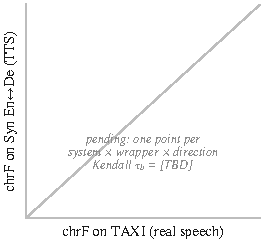
\includegraphics{figures/figA4_sim2real.pdf}
  \caption{Sim-to-real agreement: chrF of each system, wrapper and direction at its main operating point on \taxi (real speech) and on \syn \pair{En}{De} (TTS), both under L0 natural. Hollow markers: realistic wrapper; grey line: identity. Kendall's $\tau_b$, averaged over direction and wrapper strata, is annotated in the panel; its bootstrap CI is in \cref{tab:validity}.
  \protect\draftnote{placeholder; the points appear once the baselines have run on both sets}}
  \label{fig:sim2real}
\end{figure}

\paragraph{References and renders.}
To test how far silver references can rank systems, we rescore \syn \pair{En}{De} against silver references produced like the Korean ones (\cref{app:syn}) instead of the human references. To test render noise, we re-render \taxi L0 natural with seeds 1--3 under new configuration names and compare the standard deviation of chrF and \eo across seeds with the bootstrap CI width; \cref{tab:validity} lists the smallest pairwise $\tau_b$ among the three renders.

\paragraph{Metrics.}
\laal and \eo measure different waits, so a low $\tau_b$ between them is a finding rather than a validity failure: it shows that the listener's wait reorders systems. We keep \laal as the main latency metric because it was the latency metric of the IWSLT~2025 simultaneous track \citep{abdulmumin2025findings} and shares the resegmentation of our quality metrics. LongYAAL \citep{polak2025better}, computed on SoftSegmenter resegmentation in OmniSTEval and designed against the segmentation-related bias of resegmented latency, was the primary latency metric of IWSLT~2026, which reported \laal for comparison \citep{adelani2026speech}; we report how well the two agree. Rankings by string metrics alone can mislead \citep{kocmi2021ship}, which favours COMET, but the TAXI references are lowercase and unpunctuated. COMET is therefore primary on \taxi only if the lower CI bound of $\tau_b$ between its ranking and that of chrF reaches $\tau^\ast$; otherwise chrF is.
\draftnote{planned: every row of \cref{tab:validity} and the points of \cref{fig:sim2real}}
